\documentclass[sans]{beamer}
\usetheme{metropolis}
\usecolortheme{crane}

\usepackage[linesnumbered,ruled,vlined]{algorithm2e} 
\usepackage{lmodern}
\usepackage{tikz}
\usepackage{pdfpages}
\usepackage{listings}
\usepackage{multirow}
\usepackage[utf8]{inputenc}
\usepackage{graphicx}
\usepackage{ulem}
\usetikzlibrary{arrows, positioning, shapes.geometric}
\usetikzlibrary{shadows.blur}
\usetikzlibrary{decorations.pathmorphing}

% hide the footline navigation
\setbeamertemplate{footline}[frame number]{}
\setbeamertemplate{navigation symbols}{}
%\setbeamertemplate{footline}{}

\tikzset{snake it/.style={decorate, decoration=snake}}

\tikzset{
    %Define standard arrow tip
    >=stealth',
}

\tikzset{
    invisible/.style={opacity=0,text opacity=0},
    visible on/.style={alt=#1{}{invisible}},
    alt/.code args={<#1>#2#3}{%
      \alt<#1>{\pgfkeysalso{#2}}{\pgfkeysalso{#3}}
    },
}

\tikzset{
  setstyle/.style={#1},
  %bcg/.default={white},
  setstyle on/.style={alt=#1{}{setstyle}},
}

\tikzset{
  background fill/.style={fill=#1},
  background fill/.default={white},
  fill on/.style={alt=#1{}{background fill}},
}

\tikzset{
  background draw/.style={draw=#1},
  background draw/.default={white},
  draw on/.style={alt=#1{}{background draw}},
}

\tikzset{
  background filldraw/.style 2 args={draw=#1, fill=#2},
  background filldraw/.default={white}{white},
  filldraw on/.style={alt=#1{}{background filldraw}},
}

\tikzset{
  background shade/.style={#1},
  background shade/.default={top color=white, bottom color=white},
  shade on/.style={alt=#1{}{background shade}},
}

\tikzset{
  background shadedraw/.style 2 args={draw=#1, #2},
  background shadedraw/.default={white}{top color=white, bottom color=white},
  shadedraw on/.style={alt=#1{}{background shadedraw}},
}

\definecolor{darkgreen}{rgb}{0.0, 0.6, 0.13}

 \lstset{escapeinside={<@}{@>}, columns=fullflexible, basicstyle=\ttfamily}

 \title{\fontsize{0.905em}{1.5em}\selectfont Symbiotic: finding bugs in C programs}
 \author{
 {Marek~Chalupa}
 }
 \bigskip
 \institute {DevConf 2019 , 25. 1. 2019}
 \date{~\\[1cm]}

\begin{document}

%% -------------------------------------------------------------------
\maketitle
%% -------------------------------------------------------------------

%% -------------------------------------------------------------------
\begin{frame}
\frametitle{Bugs}
\begin{itemize}
  \item Bugs are annoying (if nothing else...).
  \item Nowadays, we usually use testing to find them.
  \item It is hard to write tests that reveal bugs.
  \item Automatic test generation can be used.
\end{itemize}
\end{frame}
%% -------------------------------------------------------------------


%% -------------------------------------------------------------------
\begin{frame}
\frametitle{Symbolic Execution}
\begin{itemize}
  \item Given a program with inputs:
  \begin{itemize}
    \item use symbols instead of inputs,
    \item execute the program with these symbols,
    \item fork the execution on branchings.
  \end{itemize}
  \item This way we can enumerate all possible paths in the program.
\end{itemize}
\end{frame}
%% -------------------------------------------------------------------

%% -------------------------------------------------------------------
\begin{frame}[fragile]
\frametitle{Symbolic execution}
\begin{center}
\begin{tabular}{c}
\begin{lstlisting}[language=C]
void foo(int a, int b, int c)
{
    if (a > 0) {
        c = 2;
        if (b < 0) {
            c = b
        }
    } else {
        c = -2;
    }
    if (a + b + c <= 0)
        error();
}
\end{lstlisting}
\end{tabular}
\end{center}
\end{frame}
%% -------------------------------------------------------------------

%% -------------------------------------------------------------------
\begin{frame}[fragile]
\frametitle{Symbolic execution}
\begin{center}
\begin{tikzpicture}[
  scale=1.0,
  sibling distance=10em,
  every node/.style = {scale=1.13, shape=rectangle,
                       align=center, font=\small},
  nd/.style = {draw, font=\ttfamily\tiny,fill=white},
  cond/.style = {font=\tiny, fill=white, text=blue},
  mem/.style = {overlay, font=\tiny} ]
  \node [nd] (root) {if (a > 0);}
    child { node [nd,xshift=-4mm] {c = -2}
      child { node [nd,yshift=-14.5mm] {if (a + b + c <= 0);}
        child { node [nd] {error()}
            edge from parent node[cond,yshift=-.6mm] {$[\alpha + \beta -2 > 0]$}
        }
        child { node [nd] {}
            edge from parent node[cond] {$[\alpha + \beta -2 \le 0]$}
        }
      }
      edge from parent node[cond] {$[\alpha \le 0]$}
    }
    child { node [nd,xshift=4mm] {c = 2}
     child { node [nd, yshift=8mm]  {b < 0;}
       child { node [nd, xshift=8mm] {if (a + b + c <= 0);}
         child { node [nd] {error();}
           %edge from parent node[cond] {$[\alpha + \beta + 2 > 0]$}
         }
         edge from parent node[cond] {$[\beta \ge 0]$}
       }
       child { node [nd] {c = b;}
         child { node [nd] { if (a + b + c <= 0);}
           child { node [nd] { error();}
             edge from parent node[cond,yshift=-.5mm] {$[\alpha + \beta + \beta > 0]$}
           }
           child { node [nd] {}
             edge from parent node[cond] {$[\alpha + \beta + \beta \le 0]$}
           }
         }
         edge from parent node[cond] {$[\beta < 0]$}
       }
    }
    edge from parent node[cond] {$[\alpha > 0]$}
   }
   ;
  \node[mem, scale=1.15, yshift=.5cm, xshift=-3cm] {a := $\alpha$, b := $\beta$, c := $\gamma$};
\end{tikzpicture}
\end{center}
\end{frame}
%% -------------------------------------------------------------------

%% -------------------------------------------------------------------
\begin{frame}
\frametitle{KLEE}
\begin{itemize}
  \item Open-source symbolic executor.
  \item \url{http://klee.github.io/}
\end{itemize}
\bigskip
\begin{center}

\includegraphics[width=4cm]{klee.png}
\end{center}
\end{frame}
%% -------------------------------------------------------------------

%% -------------------------------------------------------------------
\begin{frame}[fragile]
\frametitle{KLEE}
\begin{center}
\begin{tikzpicture}[
    fl/.style = {overlay, draw, font=\ttfamily\tiny,fill=white,
                 minimum height=1cm, minimum width=0.7cm},
    bullet/.style = {overlay, draw, fill=black,
                     %minimum height=.1cm, minimum width=.1cm,
                     circle, outer sep=.5em},
  ]
  \node[fl] (source1) at (-.2, 2.3) {.c};
  \node[fl] (source2) at (0,  2.2) {.c};
  \node[fl] (source3) at (0.2,2.1) {.c};
  \node[overlay] (sources) at (0,1.5) {};
  %\node[overlay,font=\itshape] (sources) at (1,1) {sources};
  \node[fl] (test1) at (9.8 ,-2) {test};
  \node[fl] (test2) at (10  ,-2.2) {test};
  \node[fl] (test3) at (10.2,-2.4) {test};
  \node[overlay] (tests) at (10,-1.5) {};
  \node[] (llvm) at (0,0) {LLVM};
  \node[] (klee) at (10, 0) {KLEE};
  \draw[->] (llvm) -> (klee);
  \draw[->] (sources) edge (llvm);
  \draw[->] (klee) edge (tests);


\end{tikzpicture}

\end{center}
\end{frame}
%% -------------------------------------------------------------------

%% -------------------------------------------------------------------
\begin{frame}[fragile]
\frametitle{Symbiotic}
\begin{center}
\begin{tikzpicture}[
    fl/.style = {overlay, draw, font=\ttfamily\tiny,fill=white,
                 minimum height=1cm, minimum width=0.7cm},
    bullet/.style = {overlay, draw, fill=black,
                     %minimum height=.1cm, minimum width=.1cm,
                     circle, outer sep=.5em},
  ]
  \node[fl] (source1) at (-.2, 2.3) {.c};
  \node[fl] (source2) at (0,  2.2) {.c};
  \node[fl] (source3) at (0.2,2.1) {.c};
  \node[overlay] (sources) at (0,1.5) {};
  %\node[overlay,font=\itshape] (sources) at (1,1) {sources};
  \node[fl] (test1) at (9.8 ,-2) {test};
  \node[fl] (test2) at (10  ,-2.2) {test};
  \node[fl] (test3) at (10.2,-2.4) {test};
  \node[overlay] (tests) at (10,-1.5) {};
  \node[] (llvm) at (0,0) {LLVM};
  \node[] (klee) at (10, 0) {KLEE};
  \draw[->] (llvm) -> (klee);
  \draw[->] (sources) edge (llvm);
  \draw[->] (klee) edge (tests);

\pause
  \node[bullet] (opt1-bullet) at (2,0) {};
  \node[overlay,align=center] (opt1) at (2,-2) {code\\optimizations};
  \draw[->, dashed,overlay] (opt1) -> (opt1-bullet);

\pause
  \node[bullet] (slicing-bullet) at (6,0) {};
  \node[overlay,align=center] (slicing) at (6,2) {program\\slicing};
  \draw[->, dashed,overlay] (slicing) -> (slicing-bullet);
\end{tikzpicture}
\end{center}
\end{frame}
%% -------------------------------------------------------------------

%% -------------------------------------------------------------------
\begin{frame}
\frametitle{Program Slicing}
\begin{itemize}
  \item Compute dependencies between instructions.
  \item We say that instruction A depends on instruction B if:
  \begin{itemize}
    \item instruction A uses memory that has been written by instruction~B, or
    \item instruction A may not be executed if at B we go the other way
  \end{itemize}
  %\item We must perform pointer analysis to correctly compute dependencies.
  \item Slicing: keep only the instructions on which the error (transitively) depends.
\end{itemize}
\end{frame}
%% -------------------------------------------------------------------

%% -------------------------------------------------------------------
\begin{frame}
\frametitle{Program Slicing -- Example}
Example!
\end{frame}
%% -------------------------------------------------------------------



%% -------------------------------------------------------------------
\begin{frame}[fragile]
\frametitle{Symbiotic - cont.}
\begin{center}
\begin{tikzpicture}[
    fl/.style = {overlay, draw, font=\ttfamily\tiny,fill=white,
                 minimum height=1cm, minimum width=0.7cm},
    bullet/.style = {overlay, draw, fill=black,
                     %minimum height=.1cm, minimum width=.1cm,
                     circle, outer sep=.5em},
  ]
  \node[fl] (source1) at (-.2, 2.3) {.c};
  \node[fl] (source2) at (0,  2.2) {.c};
  \node[fl] (source3) at (0.2,2.1) {.c};
  \node[overlay] (sources) at (0,1.5) {};
  %\node[overlay,font=\itshape] (sources) at (1,1) {sources};
  \node[fl] (test1) at (9.8 ,-2) {test};
  \node[fl] (test2) at (10  ,-2.2) {test};
  \node[fl] (test3) at (10.2,-2.4) {test};
  \node[overlay] (tests) at (10,-1.5) {};
  \node[] (llvm) at (0,0) {LLVM};
  \node[] (klee) at (10, 0) {KLEE};
  \draw[->] (llvm) -> (klee);
  \draw[->] (sources) edge (llvm);
  \draw[->] (klee) edge (tests);

  \node[bullet] (opt1-bullet) at (2,0) {};
  \node[overlay,align=center] (opt1) at (2,-2) {code\\optimizations};
  \draw[->, dashed,overlay] (opt1) -> (opt1-bullet);

  \node[bullet] (slicing-bullet) at (6,0) {};
  \node[overlay,align=center] (slicing) at (6,2) {program\\slicing};
  \draw[->, dashed,overlay] (slicing) -> (slicing-bullet);

\pause
  \node[bullet] (instr-bullet) at (4,0) {};
  \node[overlay,align=center] (instr) at (4,2) {find\\possible errors};
  \draw[->, dashed,overlay] (instr) -> (instr-bullet);

\pause
  \node[bullet] (opt2-bullet) at (8,0) {};
  \node[overlay,align=center] (opt2) at (8,-2) {code\\optimizations};
  \draw[->, dashed,overlay] (opt2) -> (opt2-bullet);

\end{tikzpicture}
\end{center}
\end{frame}
%% -------------------------------------------------------------------




%% -------------------------------------------------------------------
\begin{frame}
\frametitle{Symbiotic -- cont.}
\begin{itemize}
  \item Apart from the already mentioned steps, Symbiotic:
  \begin{itemize}
    \item automatically marks memory symbolic,
    \item replaces undefined functions with symbolic stubs.
  \end{itemize}
  \item Limits: no C++ (exceptions), no threads (yet).
  %\item Provides model of the environment (libc, POSIX).
\end{itemize}
\end{frame}
%% -------------------------------------------------------------------

%% -------------------------------------------------------------------
\begin{frame}
\frametitle{Future Directions}
\begin{itemize}
  \item Scalability
  \begin{itemize}
    \item slicing (faster analyses),
    \item symbolic execution (abstraction).
  \end{itemize}
  \item Better modelling of the environment (POSIX).
  \item Nicer representation of the results.
  \item C++ and threads.
\end{itemize}
\end{frame}
%% -------------------------------------------------------------------

%% -------------------------------------------------------------------
\begin{frame}
\frametitle{Conclusion}
\begin{itemize}
  \item Symbiotic is a tool for finding bugs in C programs.
  \item Combines fast static analysis with program slicing and symbolic execution.
  \item Runs on sequential C code.
  \item Still needs some work
  \begin{itemize}
    \item scalability issues,
    \item no C++ and threads
  \end{itemize}
\end{itemize}

\pause
\bigskip
\begin{center}
\url{https://github.com/staticafi/symbiotic}
\end{center}
\bigskip
\hfill Thank you!


\end{frame}
%% -------------------------------------------------------------------
\end{document}
